\section{Icke sinusformade signaler}
\textbf{HAREC a.\ref{HAREC.a.1.7}\label{myHAREC.a.1.7}}

\subsection{Grundton, övertoner- Kantvågor}
\textbf{HAREC a.\ref{HAREC.a.1.7.2}, a.\ref{HAREC.a.1.7.3}, a.\ref{HAREC.a.1.7.4b}\label{myHAREC.a.1.7.2}\label{myHAREC.a.1.7.3}\label{myHAREC.a.1.7.4b}}

\begin{figure*}
\begin{center}
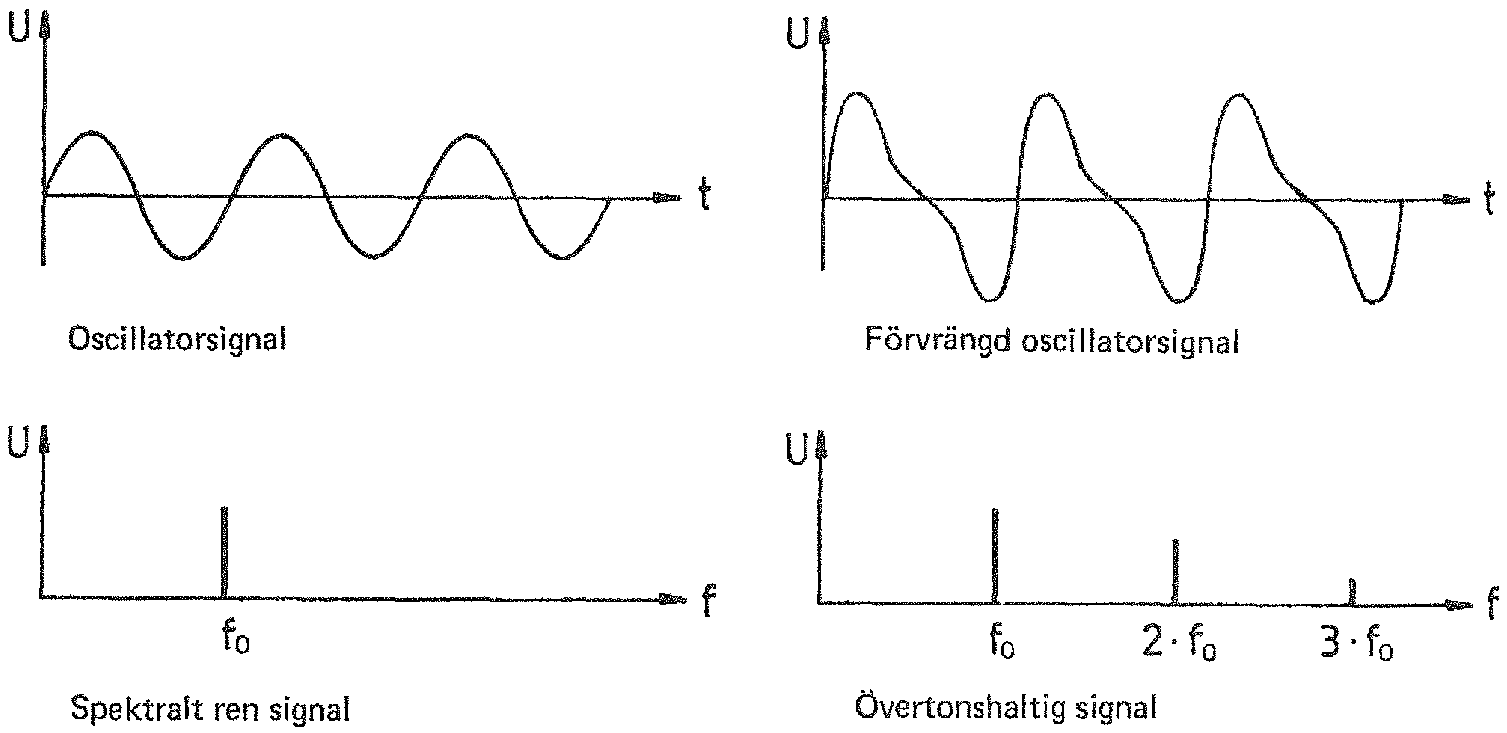
\includegraphics[width=14cm]{images/bild_2_1-18}
\caption{Ren sinusvåg och övertonshaltig våg}
\label{fig:BildII1-18}
\end{center}
\end{figure*}

Bild \ref{fig:BildII1-18}.

Ett sinusformat förlopp med en enda frekvens - en enda ton - sägs vara
spektralt ren. En sådan svängning kallas för grundton.

Varje signal, som inte är sinusformad, är sammansatt av flera sinussvängningar.
Det är signalens grundton samt dess harmoniska övertoner, vilka kan ha 2, 3
o.s.v. gånger högre frekvens än grundtonen. Den inbördes styrkan på grundton
och övertoner avgör signalens form. Om signalen ligger inom det hörbara
området, kan man märka hur den ändrar karaktär beroende på övertonshalten. Man
kan säga att övertonerna modulerar grundtonen.

\begin{figure*}
\begin{center}
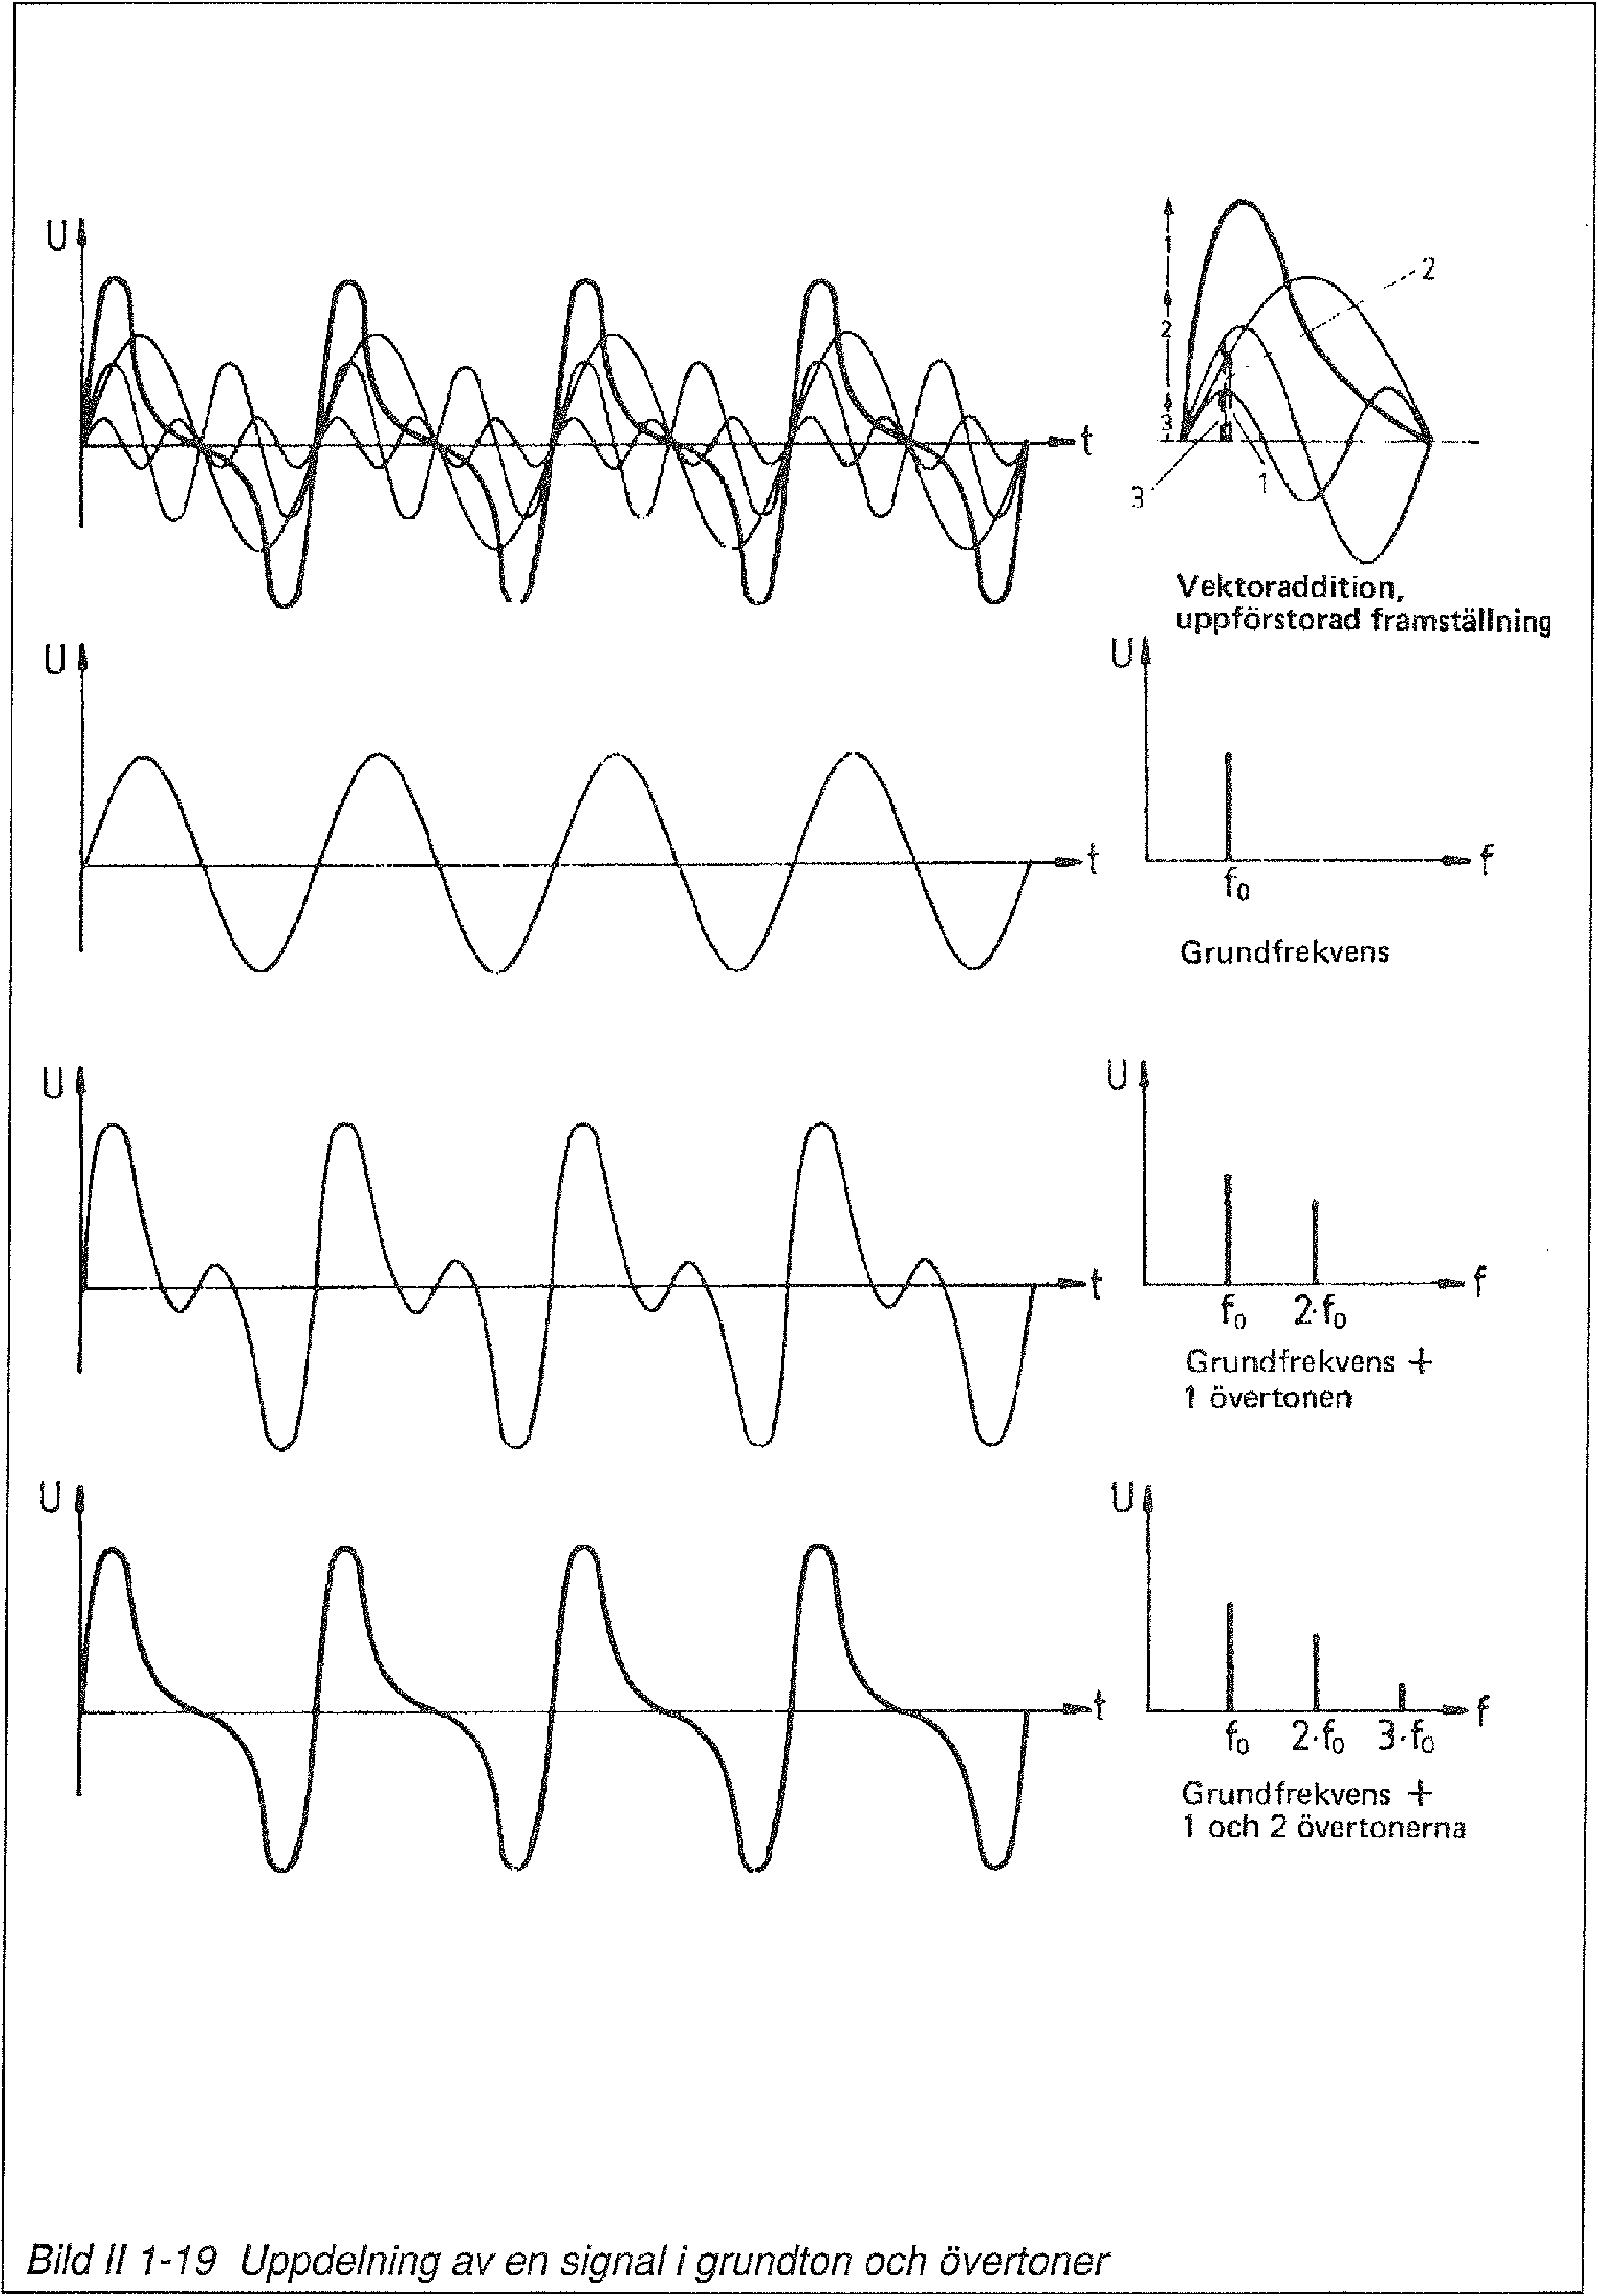
\includegraphics[width=14cm]{images/bild_2_1-19}
\caption{Uppdelning av en signal i grundton och övertoner}
\label{fig:BildII1-19}
\end{center}
\end{figure*}

Bild \ref{fig:BildII1-19}.

Oscillatorsignalen i exemplet på bilden har 1 volts amplitud på grundtonen
\(f_0\) (1:a harmoniska), 0.7 volts amplitud på de 1:a övertonen
(2:a harmoniska) och 0.2 volts amplitud på den 2:a övertonen (3:e harmoniska).
Den totala amplituden blir emellertid inte summan av 1, 0.7 och 0.2 volt
eftersom de olika delspänningarnas toppvärden inte uppträder samtidigt.
I stället måste delspänningarna adderas vid varje tidpunkt för sig.

\begin{figure*}
\begin{center}
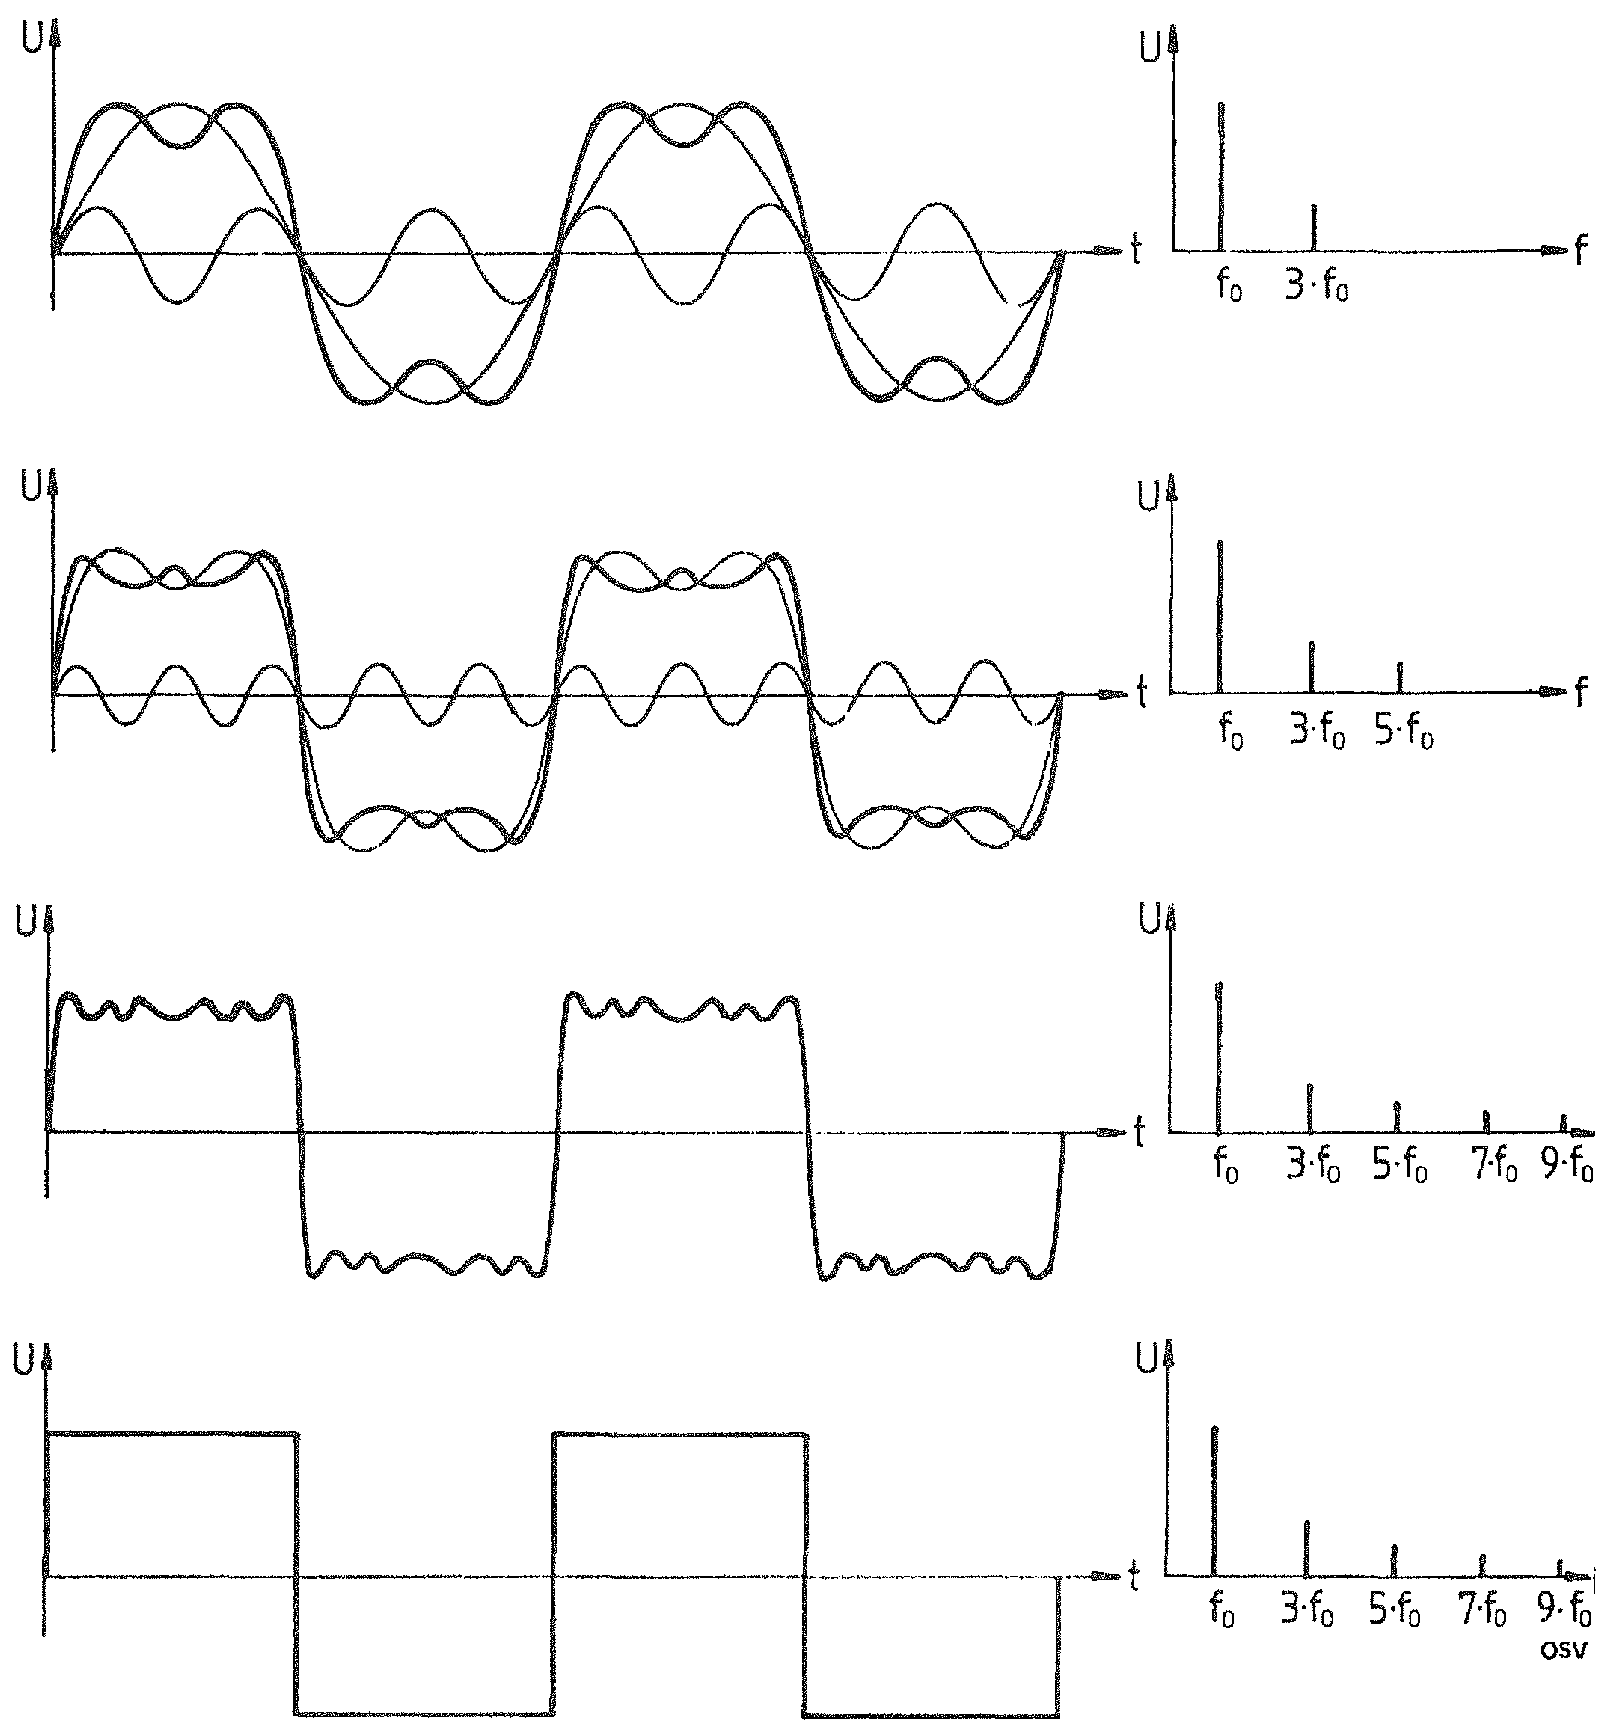
\includegraphics[width=14cm]{images/bild_2_1-20}
\caption{Uppdelning av en fyrkantvåg i grundton och övertoner}
\label{fig:BildII1-20}
\end{center}
\end{figure*}

Bild \ref{fig:BildII1-20}.

Det finns olika karaktärer av förlopp såsom sinusvåg, triangelvåg, sågtandsvåg,
fyrkantvåg o.s.v.

Fyrkantvågen är sammansatt av sinusvågor med grundfrekvensen och dess udda
övertoner, varvid amplituderna fördelar sig som \(1/1\), \(1/3\), \(1/5\),
\(1/7\), \(1/9\), \(1/11\) o.s.v. Teoretiskt når övertonsspektrum upp till
oändligt höga frekvenser, medan de motsvarande amplituderna minskar till
oändligt små värden.

En ideal fyrkantvåg, vilken inte kan uppnås i praktiken, skulle bestå av ett
oändligt antal udda övertoner med fallande amplitud. Ju fler av de högre
övertonerna som filtreras bort, desto mer lutar fyrkantvågens flanker, desto
rundare blir hörnen på vågen och desto vågigare blir kurvans topp.

\subsection{Överlagrade spänningar
(likspänningskomposant)}
\textbf{HAREC a.\ref{HAREC.a.1.7.4a}\label{myHAREC.a.1.7.4a}}

\begin{figure*}
\begin{center}
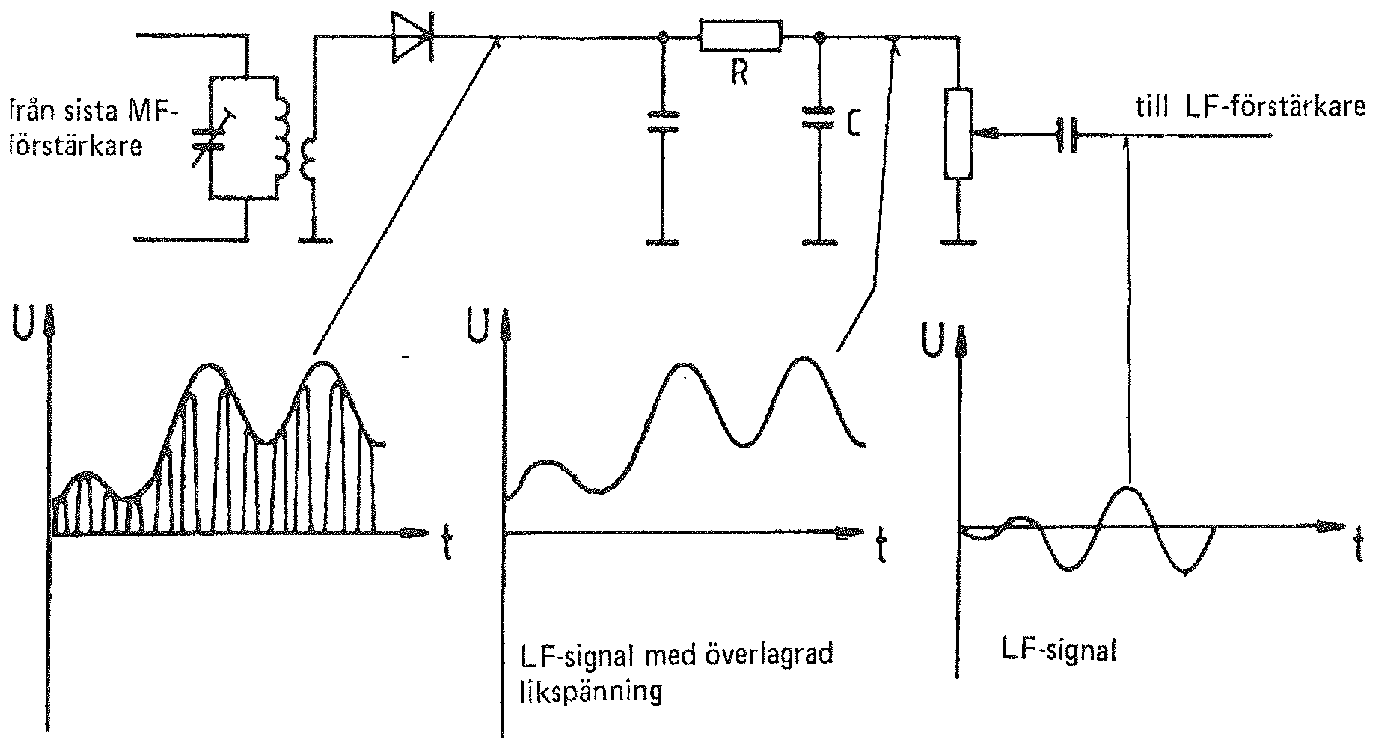
\includegraphics[width=14cm]{images/bild_2_1-21}
\caption{Överlagrade spänningar}
\label{fig:BildII1-21}
\end{center}
\end{figure*}

Bild \ref{fig:BildII1-21}.

I signalkretsar förekommer det mycket ofta, att växelspänning överlagras på likspänning
eller omvänt. Likspänningen kallas då för likspänningskomposant. Olika åtgärder behövs för
att överlagra spänningar på varandra och att sedan skilja dem åt.

Bilden visar ett avsnitt av en AM-mottagare. Från vänster hämtas en AM-modulerad signal
från MF-förstärkaren för att demoduleras, d.v.s. för att återvinna den modulerande
LF-signalen. MF-signalen halvvågslikriktas. Kvar blir den positiva delen av MF-signalen
och den modulerande LF-signalen, sammanlagrade. LF-signalen skall nu skiljas ut och
förstärkas. Alltså filtreras MF-komposanten bort. Kvar blir LF-signalen, men överlagrad på
en likspänning. Likspänningen stoppas och kvar blir slutligen LF-signalen som förstärks.
